\subsection{Testing}

\subsubsection{Analisi Statica - CodeMR}
\subsubsection{Analisi Dinamica - JUnit}

\begin{figure}[H]
    \centering
    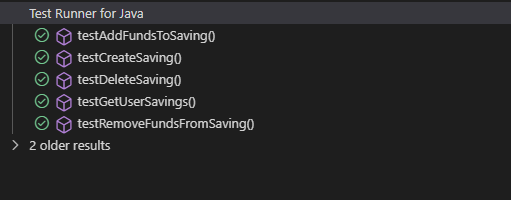
\includegraphics[width=0.9\textwidth]{images/SavingServiceTest.png}
    \caption{Test per la classe SavingService}
    \label{fig:SavingServiceTest}
\end{figure}

\begin{figure}[H]
    \centering
    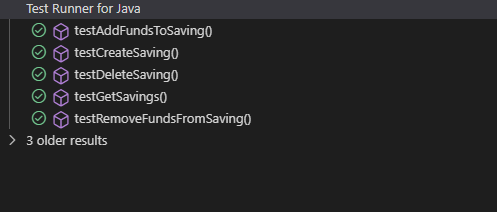
\includegraphics[width=0.9\textwidth]{images/SavingControllerTest.png}
    \caption{Test per la classe SavingController}
    \label{fig:SavingControllerTest}
\end{figure}

\begin{figure}[H]
    \centering
    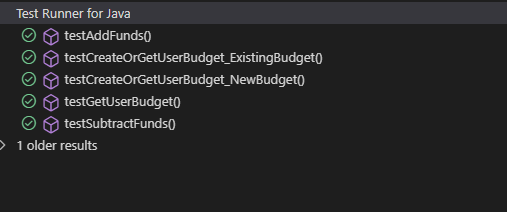
\includegraphics[width=0.9\textwidth]{images/BudgetServiceTest.png}
    \caption{Test per la classe BudgetService}
    \label{fig:BudgetServiceTest}
\end{figure}

\begin{figure}[H]
    \centering
    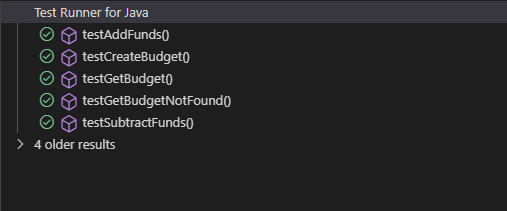
\includegraphics[width=0.9\textwidth]{images/BudgetControllerTest.png}
    \caption{Test per la classe BudgetController}
    \label{fig:BudgetControllerTest}
\end{figure}

\subsubsection{API}

\paragraph{Crea di un budget} 

\begin{itemize}
    \item \textbf{Endpoint:} \texttt{POST /api/budget/create}
    \item \textbf{Descrizione:} Permette all'utente creare un nuovo Budget.
    \item \textbf{Parametri:}
    \begin{itemize}
        \item \texttt{username} (String) - Username utente.
        \item \texttt{amount} (duble) - Valore budget.
    \end{itemize}
\end{itemize}

\begin{figure}[H]
    \centering
    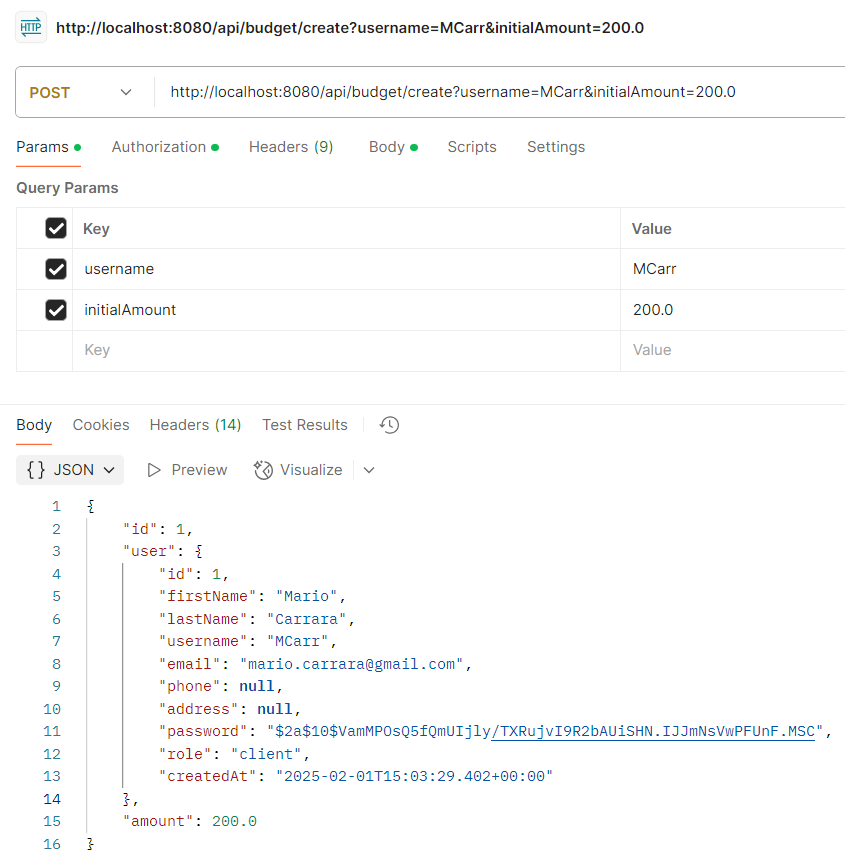
\includegraphics[width=0.9\textwidth]{images/CreateBudgetAPI.png}
    \caption{API creazione budget}
    \label{fig:CreateBudgetAPI}
\end{figure}

\paragraph{Visualizza budget utente} 

\begin{itemize}
    \item \textbf{Endpoint:} \texttt{GET /api/budget}
    \item \textbf{Descrizione:} Permette di ottenere il budget di un utente.
    \item \textbf{Parametri:}
    \begin{itemize}
        \item \texttt{username} (String) - Username utente.
    \end{itemize}
\end{itemize}

\begin{figure}[H]
    \centering
    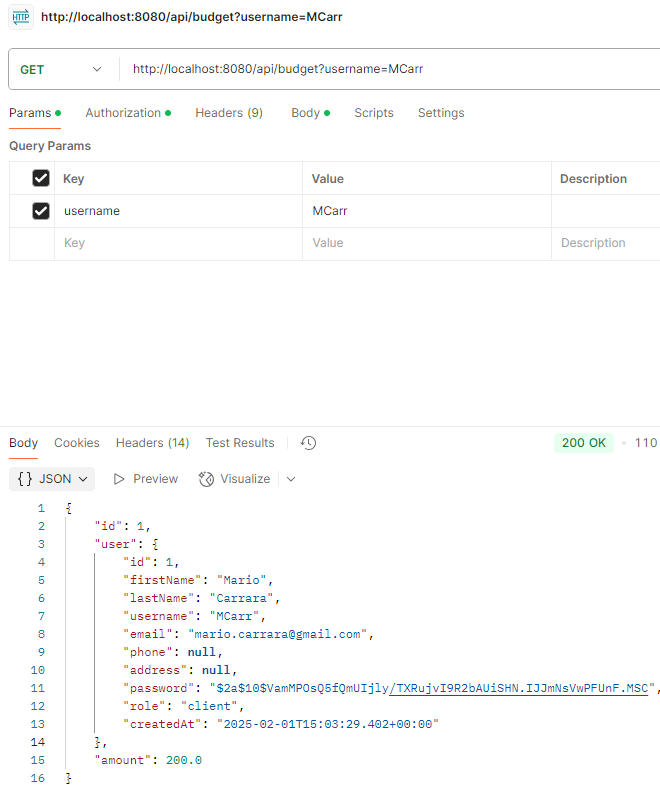
\includegraphics[width=0.9\textwidth]{images/GetBudgetAPI.png}
    \caption{API visualizza budget di un utente}
    \label{fig:GetBudgetAPI}
\end{figure}

\paragraph{Incrementa budget} 

\begin{itemize}
    \item \textbf{Endpoint:} \texttt{PUT /api/budget/add}
    \item \textbf{Descrizione:} Permette di incrementare il valore  del budget
    \item \textbf{Parametri:}
    \begin{itemize}
        \item \texttt{username} (String) - Username utente.
        \item \texttt{amount} (duble) - Valore da aggiungere al budget.
    \end{itemize}
\end{itemize}

\begin{figure}[H]
    \centering
    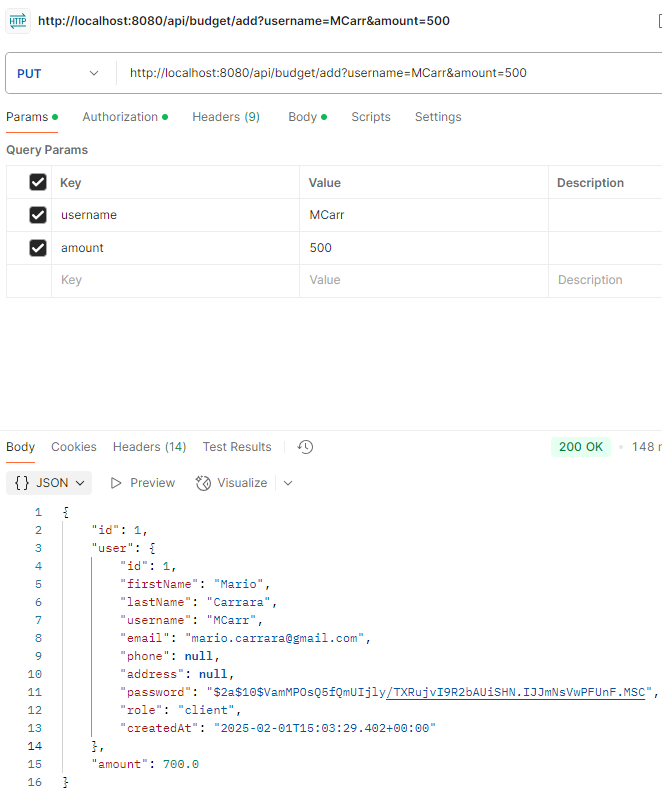
\includegraphics[width=0.9\textwidth]{images/AddBudgetAPI.png}
    \caption{API per aggiungere fondi al budget}
    \label{fig:AddBudgetAPI}
\end{figure}

\paragraph{Decrementa budget} 

\begin{itemize}
    \item \textbf{Endpoint:} \texttt{PUT /api/budget/subtract}
    \item \textbf{Descrizione:} Permette di incrementare il valore  del budget
    \item \textbf{Parametri:}
    \begin{itemize}
        \item \texttt{username} (String) - Username utente.
        \item \texttt{amount} (duble) - Valore da sottrarre al budget.
    \end{itemize}
\end{itemize}

\begin{figure}[H]
    \centering
    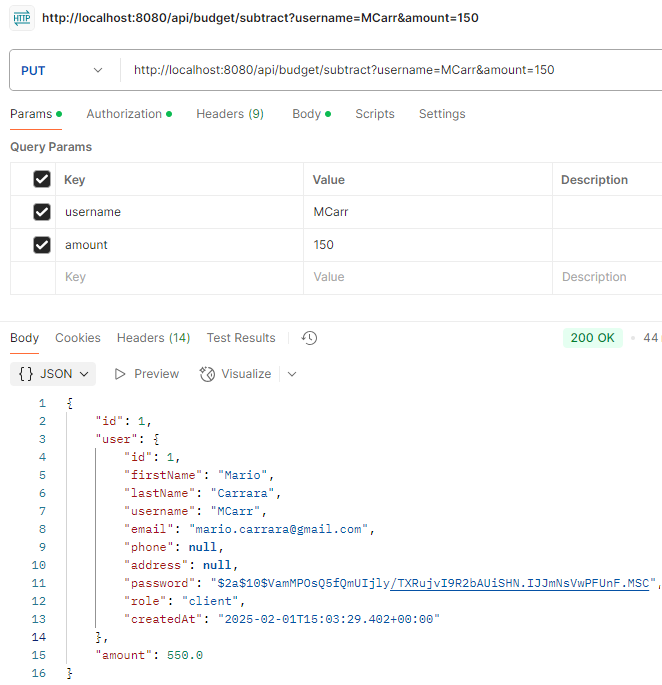
\includegraphics[width=0.9\textwidth]{images/SubtractBudgetAPI.png}
    \caption{API per sottrarre fondi al budget}
    \label{fig:SubtractBudgetAPI}
\end{figure}

\paragraph{Crea risparmio} 

\begin{itemize}
    \item \textbf{Endpoint:} \texttt{POST /api/savings/create}
    \item \textbf{Descrizione:} Permette di creare un risparmio
    \item \textbf{Parametri:}
    \begin{itemize}
        \item \texttt{username} (String) - Username utente.
        \item \texttt{name} (String) - Nome del risparmio
        \item \texttt{amount} (duble) - Valore del risparmio
    \end{itemize}
\end{itemize}

\begin{figure}[H]
    \centering
    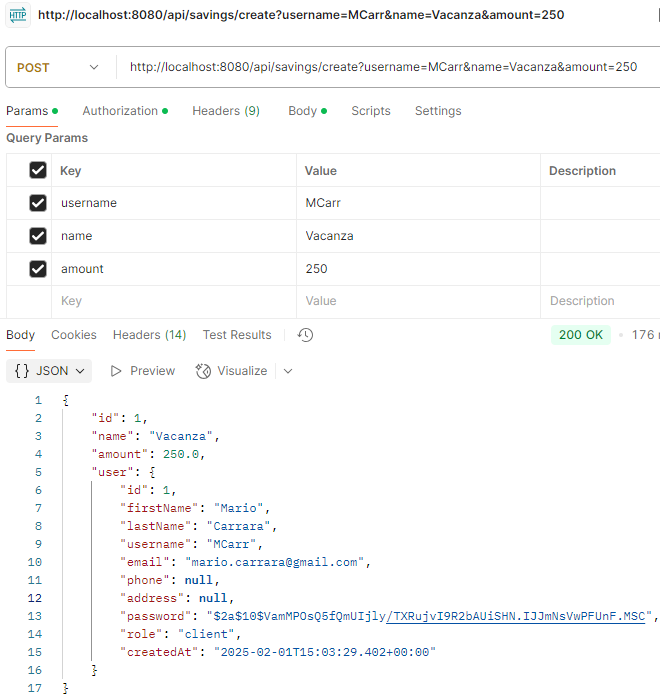
\includegraphics[width=0.9\textwidth]{images/CreateSavingAPI.png}
    \caption{API per creare un risparmio}
    \label{fig: CreateSavingAPI}
\end{figure}

\paragraph{Visualizza risparmi utente} 

\begin{itemize}
    \item \textbf{Endpoint:} \texttt{GET /api/savings}
    \item \textbf{Descrizione:} Permette di ottenere i risparmi degll'utente
    \item \textbf{Parametri:}
    \begin{itemize}
        \item \texttt{username} (String) - Username utente.
    \end{itemize}
\end{itemize}

\begin{figure}[H]
    \centering
    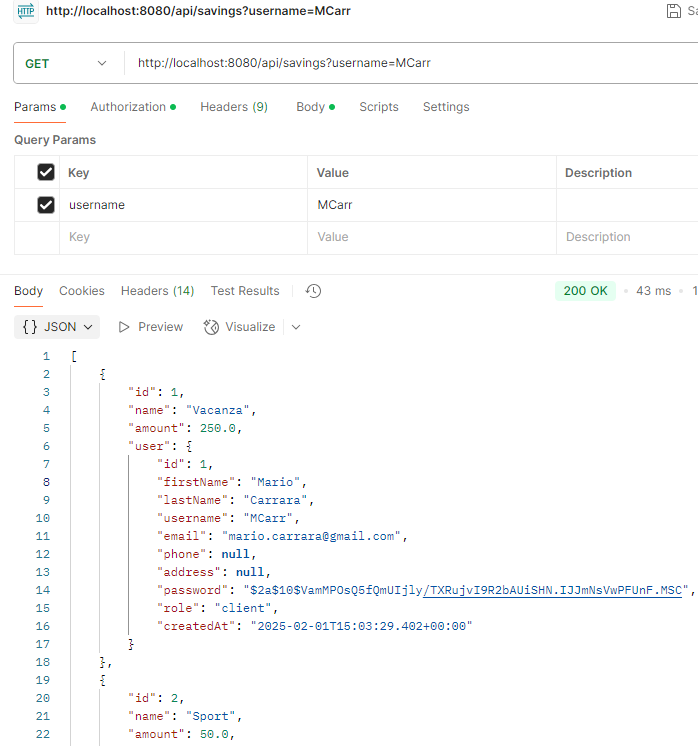
\includegraphics[width=0.9\textwidth]{images/GetSavingsAPI.png}
    \caption{API per ottenere i risparmi dell'utente}
    \label{fig: GetSavingAPI}
\end{figure}

\paragraph{Aggiungi fondo al risparmio} 

\begin{itemize}
    \item \textbf{Endpoint:} \texttt{PUT /api/savings/addFunds}
    \item \textbf{Descrizione:} Permette di aggiungere fondi ai risparmi degli utenti.
    \item \textbf{Parametri:}
    \begin{itemize}
        \item \texttt{username} (String) - Username utente.
        \item \texttt{savingId} (Long) - Id del risparmio.
        \item \texttt{amount} (double) - Valore da aggiungere al risparmio.
    \end{itemize}
\end{itemize}

\begin{figure}[H]
    \centering
    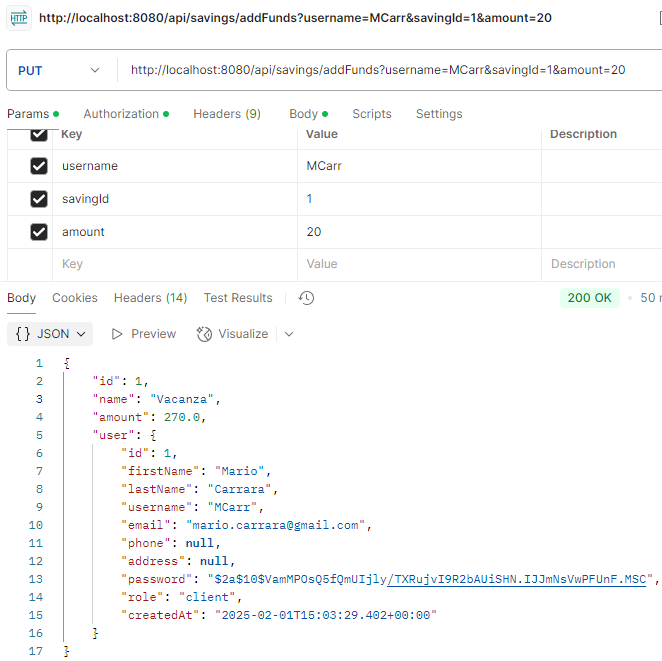
\includegraphics[width=0.9\textwidth]{images/AddFundsSavingAPI.png}
    \caption{API per aggiungere fondi ai risparmi dell'utente}
    \label{fig:AddFundsSavingAPI}
\end{figure}

\paragraph{Rimuovi fondo al risparmio} 


\begin{itemize}
    \item \textbf{Endpoint:} \texttt{PUT /api/savings/removeFunds}
    \item \textbf{Descrizione:} Permette di togliere fondi ai risparmi degli utenti.
    \item \textbf{Parametri:}
    \begin{itemize}
        \item \texttt{username} (String) - Username utente.
        \item \texttt{savingId} (Long) - Id del risparmio.
        \item \texttt{amount} (double) - Valore da togliere al risparmio.
    \end{itemize}
\end{itemize}

\begin{figure}[H]
    \centering
    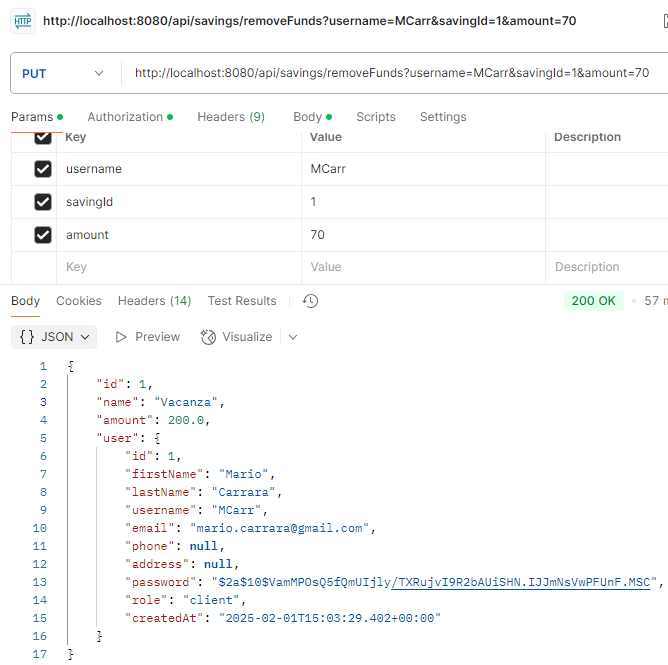
\includegraphics[width=0.9\textwidth]{images/RemoveFundsSavingAPI.png}
    \caption{API per togliere fondi ai risparmi dell'utente}
    \label{fig:RemoveFundsSavingAPI}
\end{figure}

\paragraph{Elimina risparmio}

\begin{itemize}
    \item \textbf{Endpoint:} \texttt{DELETE /api/savings/delete}
    \item \textbf{Descrizione:} Permette di eliminare un risparmio.
    \item \textbf{Parametri:}
    \begin{itemize}
        \item \texttt{username} (String) - Username utente.
        \item \texttt{savingId} (Long) - Id del risparmio.
    \end{itemize}
\end{itemize}

\begin{figure}[H]
    \centering
    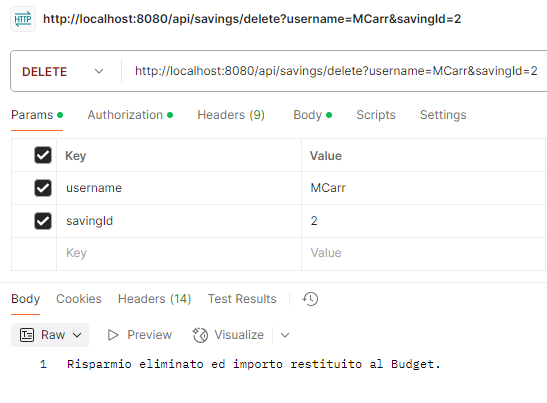
\includegraphics[width=0.9\textwidth]{images/DeleteSavingAPI.png}
    \caption{API per eliminare un risparmio}
    \label{fig:DeleteSavingAPI}
\end{figure}